\section{Экспериментальная установка}
Принципиальная схема релаксометра ЯМР, согласно описанию из \ref{met:1} приведена на рис. \ref{fig:installation}

\begin{figure}[h]
	\centering
	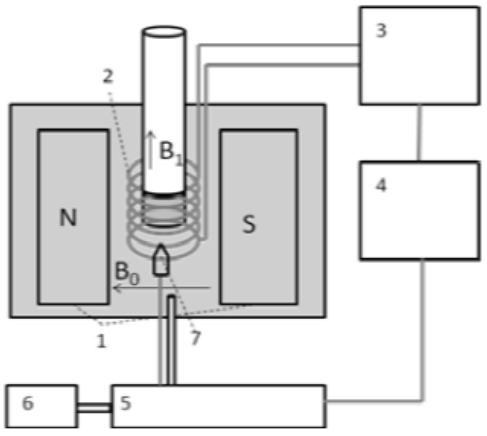
\includegraphics[width=0.6\linewidth]{Installation}
	\caption{Принципиальная схема: \textbf{1} -- постоянный магнит; \textbf{2} -- приемопередающая катушка; \textbf{3} -- генератор импульсов и приемник излучения; \textbf{4} -- компьютер; \textbf{5} -- система термостатирования образца (\textit{на установке отсутствовала}); \textbf{6} -- воздушный компрессор; \textbf{7} -- термопара}
	\label{fig:installation}
\end{figure}

Основной частью ЯМР-релаксометра является магнит (\textbf{1} на рис. \ref{fig:installation}), создающий постоянное магнитное поле напряженностью $ \vec{B}_0 $. Величина напряженности постоянного МП релаксометра \textit{Bruker minispec}, используемого в этой работе, составляет около $ 0.5 $ Тл ($ 5 \cdot 10^3 $ Гс). Этой напряженности соответствует рабочая частота для протонов $ \nu_0 = 20 $ МГц.

Переменное магнитное поле, перпендикулярное постоянному магнитному полю, создается при помощи катушки индуктивности, вдоль оси которой располагается пробирка с исследуемым образцом. Параллельно катушке включен конденсатор так, что образованный радиочастотный контур настроен на резонансную ларморовскую частоту.

Для созданя импульсов переменного поля катушка \textbf{2} соединяется с радиочастотным генератором, расположенным в \textbf{3}. Слабый сигнал ЯМР предварительно усиливается, затем поступает в блок управляющей электроники, где и производится его детектирование. При этом следует учитывать наличие переходных процессов в приемном контуре и усилителе, из-за которых у приемника существует т.н. <<мертвое время>> порядка 100 нс, необходимое для переключения в режим приема и усиления слабого сигнала намагниченности после периода генерации мощных импульсов.

\section{Эксперимент}
\subsection{Ход работы}
\begin{enumerate}
	\item Настройка и проверка прибора
	\item Регистрация времен $T_2^*, T_2, T_1$ для дистиллированной воды
	\item \label{exp:routine-1} Приготовление раствора соли (изначально $MnSO_4$) заданной концентрации
	\item \label{exp:routine-2} Регистрация времен $T_2^*, T_2, T_1$ для полученного раствора
	\item Повторение пунктов \ref{exp:routine-1}), \ref{exp:routine-2}) для 3 концентраций $MnSO_4$ и 2 концентраций $Na_2SO_4$.
\end{enumerate}
Для измерения использовалась программа \textit{Bruker the minispec}.